\chapter{Funzioni Hash}
Una funzione hash è una funzione che comprime e questo fa sì che un input di lunghezza arbitraria si trasformi in un output di lunghezza fissata. Un'importante caratteristica di queste funzioni sono le così dette \textbf{collisioni}. 
Definiamo una collisione per $H:D\xrightarrow{} R$ una coppia tale che $H(x_1)=H(x_2)$ con $x_1 \neq x_2$.

Naturalmente se dovessimo avere che $|D| > |R|$ le collisioni sarebbero inevitabili per il teorema del \textbf{pigeon hole}. Diremo che H è \textbf{resistente alle collisioni} se è computazionalmente impossibile trovare delle collisioni. Considereremo una famiglia di funzioni 
\[H:\{0,1\}^k \times D \xrightarrow{} \{0,1\}^n\]
Per cui, fissata una chiave k, si definisce $h(x)=H_k(x)$. 

Definiamo una funzione H \textbf{Universale o Quasi Universale} se il vantaggio $Adv^{cr0}(A) = Pr[Esp_H^{cr0}(A)=1]$ è prossimo a 0 per tutti i possibili avversari esistenti. L'esperimento considerato è questo:
\begin{figure}[H]
    \centering
    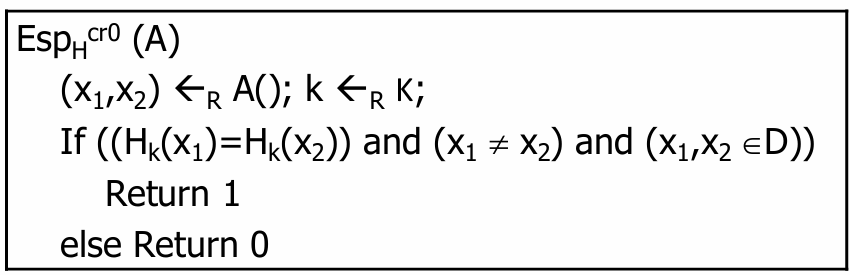
\includegraphics[width=0.5\linewidth]{Images/funzioni_hash/esp_universale.png}
\end{figure}
Notiamo come in questo caso viene semplicemente scelta una coppia a caso di input e solo dopo si fissa una chiave. 

Definiamo, invece, una funzione \textbf{Universale Unidirezionale} se il vantaggio $Adv^{cr1-kk}(A) = Pr[Esp_H^{cr1-kk}(A)=1]$ per ogni possibile avversario computazionalmente limitato nel seguente esperimento è prossimo a 0. In buona sostanza, questo vantaggio è prossimo a 0 se non è possibile, a partire da un certo hash, estrarre computazionalmente tutti gli input che danno quell'hash. 
\begin{figure}[H]
    \centering
    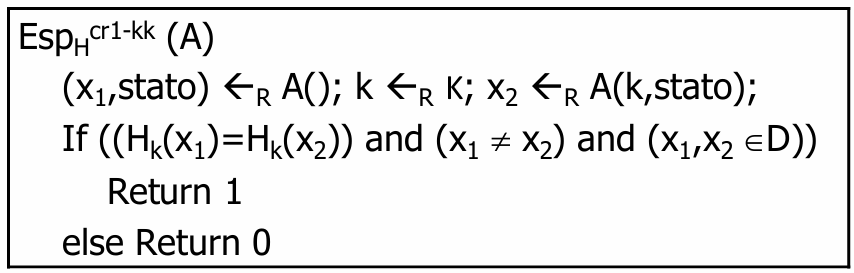
\includegraphics[width=0.5\linewidth]{Images/funzioni_hash/esp_universale_unidirezionale.png}
\end{figure}
Notiamo che l'esperimento è molto simile a quello precedente, tuttavia, la differenza sta nel fatto che prima scegliamo un input e, fissata la chiave, si sceglierà il secondo input. Abbiamo un elemento aggiuntivo in questo esperimento che viene rappresentato dalla variabile stato che non fa altro che salvare ciò che accade precedentemente. 

Chiaramente una funzione universale unidirezionale è anche una funzione universale e ciò può essere dimostrato così:
\textbf{Ipotesi:} H è una funzione universale unidirezionale.

\textbf{Tesi:} H è una funzione universale.

Quello che vogliamo dimostrare è che avremo che l'attaccante A che attacca la funzione con l'esperimento cr1-kk limita superiormente l'attaccante B che attacca la funzione hash per universalità nell'esperimento cr0.

Immaginiamo di avere il seguente attaccante A() che non fa altro che questo:
\begin{algorithm}[H]
\caption{Attaccante A}
\begin{algorithmic}[1]
\Statex \textbf{A()}
\State $(x_1, x_2) \gets B()$ \Comment{Esegui la procedura $B()$}
\State $stato \gets x_2$ \Comment{Salva $x_2$ come stato}
\State \Return $(x_1, stato)$ \Comment{Restituisci $x_1$ e il nuovo stato}
\Statex
\Statex \textbf{Chiamata A(k, stato)}
\State $x_2 \gets stato$ \Comment{Carica lo stato precedente}
\State \Return $x_2$ \Comment{Restituisci lo stato}
\end{algorithmic}
\end{algorithm}

Calcolando le probabilità vedremo che:
\[Adv(A)=Pr[Esp^{cr1-kk}(A)=1] = Pr[Esp^{cr0}(B)=1] = Adv(B)\]
Abbiamo quindi dimostrato che l'abilità di un avversario nel rompere la proprietà di universalità è limitata dall'abilità di un avversario nel rompere la proprietà di universalità unidirezionale.

Definiamo, infine, che una funzione è resistente alle collisioni se il vantaggio $Adv^{cr2-kk}(A) = Pr[Esp_H^{cr2-kk}(A)=1]$ è prossimo a 0.
\begin{figure}[H]
    \centering
    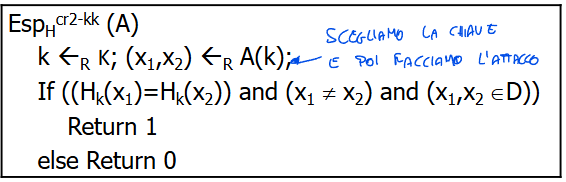
\includegraphics[width=0.7\linewidth]{Images/funzioni_hash/esp_resistente_collisioni.png}
\end{figure}

Anche in questo caso possiamo dimostrare che una funzione resistente alle collisioni è anche universale e unidirezionale. Possiamo ancora una volta dimostrarlo così:
\textbf{Ipotesi:} H è resistente alle collisioni.

\textbf{Tesi:} H è una funzione universale unidirezionale.

Supponiamo che H non sia universale unidirezionale ma che sia resistente alle collisioni. Allora esisterà un'attaccante B che attaccherà H come funzione universale unidirezionale e B sarà esattamente come era A prima. \footnote{L'attaccante dell'esperimento cr1-kk che poteva prendere come parametri nulla e poi k, stato} Vediamo cosa succede:
\begin{algorithm}[H]
\caption{Attaccante $A$}
\begin{algorithmic}[1]
\Statex \textbf{A(k)}
\State $Run B() \gets (x_1,stato$) \Comment{B attacca per u. u.}
\State $Run B(k, stato) \gets x_2$ \Comment{Runniamo nuovamente B con la chiave fissata}
\If{$H(x_1) = H(x_2)$ \textbf{and} $x_1 \neq x_2$}
    \State \Return $(x_1, x_2)$
\Else
    \State $x'_1 \gets \text{Random}()$ \Comment{Genera $x'_1$ casuale}
    \State $x'_2 \gets \text{Random}()$ \Comment{Genera $x'_2$ casuale}
    \State \Return $(x'_1, x'_2)$ 
\EndIf
\end{algorithmic}
\end{algorithm}
Calcoliamo anche in questo caso il vantaggio di A che sarà:
\[Adv(A)=Pr[Esp^{cr2-kk}(A)=1]=Pr[Esp^{cr1-kk}(B)=1]+A_{random} \geq Adv(B)\]

Ragioniamo adesso sulle chiavi, spesso noi facciamo delle affermazioni considerando una chiave non fissata, tuttavia è possibile che noi troviamo degli attacchi specifici per una singola chiave e non per tutte. Questa è una cosa che nei fatti potrebbe realmente accadere, come vedremo tra poco, tutte le funzioni hash utilizzano una chiave fissata o possono addirittura non utilizzarne una.

\section{Applicazioni di funzioni Hash}
Cerchiamo, prima di tutto, di capire a cosa servono effettivamente le funzioni Hash e perché sono così importanti al giorno d'oggi. Di fatto, senza funzioni Hash, non conosceremmo la rete per quello che è oggi e vediamo perché. 

Una delle applicazioni più conosciute è, banalmente, la verifica della password che avviene ogni qualvolta effettuiamo il login su un qualunque sito web. Nome utente e password sono salvati su un database che potrebbe essere soggetto ad attacchi per cui, se la password venissero salvate in chiaro, un qualunque hacker avrebbe nome utente e password di tutti gli utenti registrati. Utilizzando le funzioni hash ciò non accade poiché, salvando l'hash della password, anche se venisse compromesso il database, non ci sarebbe modo di ricavare la password originale.

Un'altra cosa che può essere effettuata è la verifica d'integrità di grossi file. Immaginando di voler verificare che due file di grosse dimensioni siano uguali, confrontarli bit a bit è sicuramente un'operazione dispendiosa. Una cosa molto più comoda è generare gli hash dei due file e confrontare solo quelli che, quindi, avranno dimensione minore rispetto a quella originale. 

Allo stesso modo si può agire quando si scaricano dei file da qualche sito non ufficiale controllando se l'eseguibile appena scaricato """"PAGANDO""" ha lo stesso hash dell'eseguibile ufficiale.

\section{SHA-1 (Secure Hash Algorithm 1)}
SHA-1 è una funzione di hashing tale che: 
\[SHA1:\{0,1\}^{<2^{64}} \xrightarrow{}\{0,1\}^{160}\]
Questa fu proposta nel 1995 e rimase lo standard fino al 2006 anche se, in rarissimi casi, è tutt'oggi utilizzata. L'idea alla base di questo algoritmo è quello di utilizzare una funzione di compressione che va da 512 + $l$ bit a $l$ bit soltanto. Questa idea viene comunemente chiamata \textbf{Merkle-Damgard}
Questa si compone di diverse procedure che comprendono il modificare l'input attraverso una procedura chiamata \textbf{SHAPAD} che trasforma la lunghezza del messaggio in un multiplo di 512. Dopodiché, viene iterata la funzione di compressione \textbf{shf1}.
\begin{figure}[H]
    \centering
    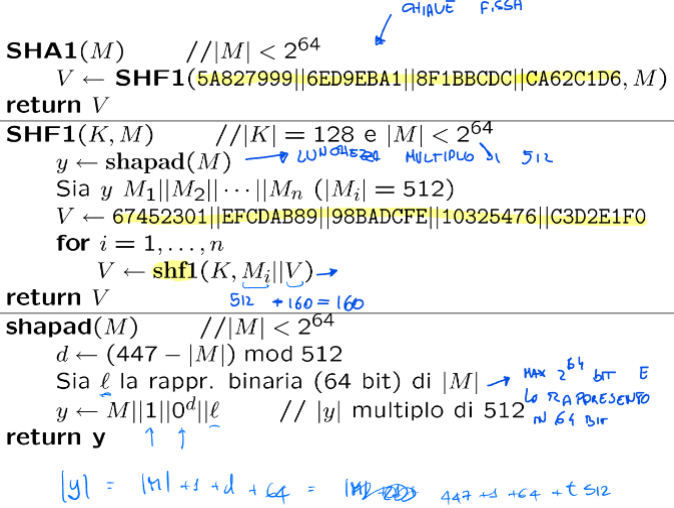
\includegraphics[width=0.7\linewidth]{Images/funzioni_hash/sha_1.png}
\end{figure}
Analizzando le procedure a grandi linee:
\begin{itemize}
    \item \textbf{SHA1(M):} Funzione principale che si occupa di fare l'hashing.
    \item \textbf{SHF1(K,M):} Questa funzione si occupa di fare il padding del messaggio, suddividerlo nei vari blocchi e, a partire dalla chiave K che è \textbf{fissa} per tutte le applicazioni di SHA1, inizia un processo che si occupa di concatenare il blocco del messaggio di 512 bit al V precedente di 160 bit per poi comprimerlo in 160 bit nuovamente in maniera da poter continuare nuovamente il processo. Ciò che verrà restituito sarà V di 160 bit che sarà l'hash del messaggio.
    \item \textbf{SHAPAD(M):} Shapad è la funzione che viene richiamata da SHF1 per effettuare il padding del messaggio e serve, per l'appunto a far sì che il messaggio abbia una lunghezza che è un multiplo di 512.
\end{itemize}

\section{Attacchi alle funzioni Hash}
Analizziamo i possibili attacchi alla proprietà di resistenza alle collisioni che è quella più utile per quanto riguarda i nostri scopi. 

L'attacco più banale che ci può venire in mente è quello di forza bruta per cui scegliamo un input a caso $x_1$ e calcoliamo il suo hash $H(x_1)$. Dopodiché, proviamo tutti i possibili $x_2$ fino a quando non abbiamo che $H(x_1)=H(x_2)$. Questo attacco avrà nel caso peggio $2^{160}$ iterazioni poiché questo è il numero dei possibili output diversi che si possono avere. 

Ripensando al paradosso del compleanno ci possiamo però immaginare uno scenario migliore rispetto ad un semplice attacco di forza bruta. Possiamo prendere due input q a caso e calcolare i rispettivi hash per cui il paradosso del compleanno sembrerebbe garantirci una complessità $O(\sqrt{|R|})$.
\begin{figure}[H]
    \centering
    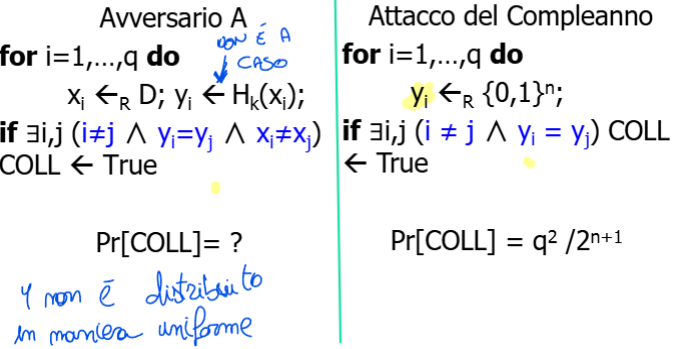
\includegraphics[width=0.7\linewidth]{Images/funzioni_hash/a_vs_compleanno.png}
\end{figure}

Notiamo però come la differenza stia proprio nel fatto che l'hash calcolato in uno specifico punto non è casuale e, inoltre, la funzione potrebbe non essere distribuita in maniera regolare. Per cui questo non sembra garantirci nulla riguardo alla possibilità di trovare la collisione. Quello che facciamo, d'altronde, non è altro che cercare una cosa di questo tipo:
\begin{figure}[H]
    \centering
    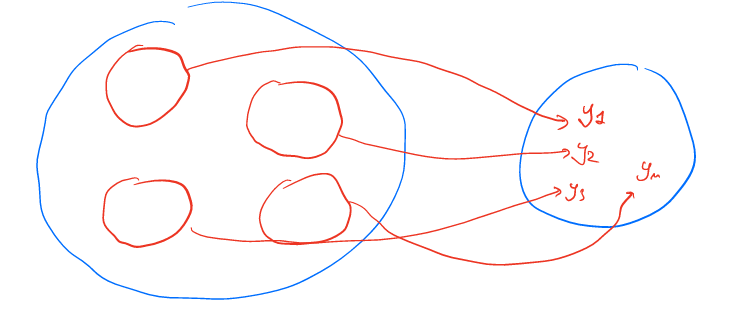
\includegraphics[width=0.7\linewidth]{Images/funzioni_hash/insiemi_hash.png}
\end{figure}
Immaginando che l'insieme più grande sia il dominio degli input, questo sarà diviso in vari sottoinsiemi che corrisponderanno a tutti gli specifici $x_i$ che danno lo stesso Hash e noi cercheremo di prendere nel pratico due elementi appartenenti allo stesso sottoinsieme. Per far sì che questa operazione sia difficile, è necessario avere quanti più sottoinsiemi possibili cosiché gli elementi che mappano lo stesso output siano pochi e ciò non dipende dalla cardinalità dell'insieme di input, bensì dalla cardinalità dell'insieme di output. Banalmente, maggiori sono gli output possibili, meglio si distribuiranno i nostri input.

L'attacco risulta ancora più efficace se la funzione non è regolare poiché se si creano sottoinsiemi più grossi di altri all'interno del dominio, sarà più facile prendere due elementi appartenenti allo stesso insieme.

\textbf{Teorema}\\
Siano:
\begin{itemize}
    \item $h: K \times \{0,1\}^{b+v} \xrightarrow{} \{0,1\}^{v}$ una famiglia di funzioni.
    \item $H: K \times D \xrightarrow{} \{0,1\}^{v}$ costruita come descritto.
    \item $A_H$ un avversario che trova collisioni in H.
\end{itemize}
Allora possiamo costruire $A_h$ che trova collisioni per h tale che:
\[Adv_H^{cr2-kk}(A_H)\leq Adv_h^{cr2-kk}(A_h)\]

Sostanzialmente ciò ci dice che se h è resistente alle collisioni, allora ciò varrà anche per H.

\section{Sponge Construction}

Questo paradigma è alternativo a Merkle Damgaard ed è un semplice processo iterativo basato su una specifica permutazione:\footnote{Come dicevamo, non abbiamo chiave}
\[P:\{0,1\}^n \xrightarrow{} \{0,1\}^n\]

Questa operazioni contiene due parametri fondamentali $r$ detto rate, $c$ detto capacity $:r+c = n$ dove n rappresenta la lunghezza della stringa. Troviamo, inoltre, $v$ che rappresenta la dimensione dell'output e $L-max$ che rappresenta la massima dimensione dei messaggi che è, in genere, $\{0,1\}^{<L+1}$.

Questo algoritmo si compone di due fasi principali:
\begin{enumerate}
    \item \textbf{Absorbing stage}: Durante questa fase aggiungiamo il padding\footnote{L'unica cosa necessaria per il padding è che sia iniettivo. Cioè, vogliamo che a messaggi diversi, tramite il padding, si arrivi a stringhe diversa} ad M per far sì che questo diventi multiplo di r, inizializziamo la stringa h a una stringa null e, a ogni blocco ottenuto dalla divisione di M, aggiungiamo c 0 in maniera tale da avere blocchi di n bit per poi, infine, applicare la permutazione allo xor tra h e il messaggio con gli 0 concatenati.
    \begin{figure}[H]
        \centering
        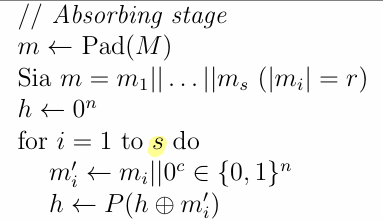
\includegraphics[width=0.5\linewidth]{Images/funzioni_hash/absorbing_stage.png}
    \end{figure}
    \item \textbf{Squeezing stage}: Una volta fatto ciò, continuiamo ad applicare la permutazione ad h e di questo prendiamo via via i primi r bit che rappresenteranno $z_i$. Il nostro output finale saranno i primi v bit della concatenazione di tutti gli z. \footnote{I bit sprecati saranno solo nell'ultimo z}
    \begin{figure}[H]
        \centering
        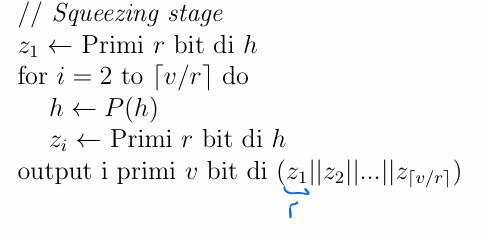
\includegraphics[width=0.7\linewidth]{Images/funzioni_hash/squeezing_stage.png}
    \end{figure}
\end{enumerate}

Lo standard NIST specifica una famiglia di funzioni Sponge-based basate sulla permutazione Keccak[c](m, v) dove c rappresenta la capacità e, generalmente, si utilizza il padding 10, m il messaggio e v la lunghezza dell'output.

